\documentclass{article}
% General document formatting
\usepackage[margin=0.7in]{geometry}
\usepackage[parfill]{parskip}
\usepackage[utf8]{inputenc}

% Related to math
\usepackage{amsmath,amssymb,amsfonts,amsthm}
\usepackage{graphicx}
\usepackage{multicol}

\title{Portfolio}
\author{Joshua Brown}

\begin{document}
\maketitle

\section*{6D Drone Pose Detection}
I made a system capable of using a cheap monocular camera to estimate the position and orientation of a drone

\begin{multicols}{2}
    \subsection*{What did I do?}
    \begin{itemize}
        \item I used a Vicon motion capture system to mark where the camera and target drone were in 3D space, and then used this setup to automatically annotate an image from the camera with points that line up with features on the drone
        \item Then I trained a keypoint RCNN machine learning model on this generated data resulting in a system that was capable of estimating feature points on a drone
        \item I then used a PnP algorithm to essentially convert the image points into a pose orientation of a target drone
    \end{itemize}
    
    \subsection*{What technologies were used?}
    \begin{itemize}
        \item \textbf{ROS2} was used for easily making all of the different processes work together as a single system
        \item \textbf{PyTorch} was used for training and using a fine-tuned keypoint RCNN model
        \item \textbf{OpenCV} was used for calibrating the intrinsic and extrinsic matrices of the camera, projecting 3D points from the motion capture system to the image for training data, and for converting estimated image points to an estimated pose
    \end{itemize}
    \vspace{10cm}
    \begin{center}
        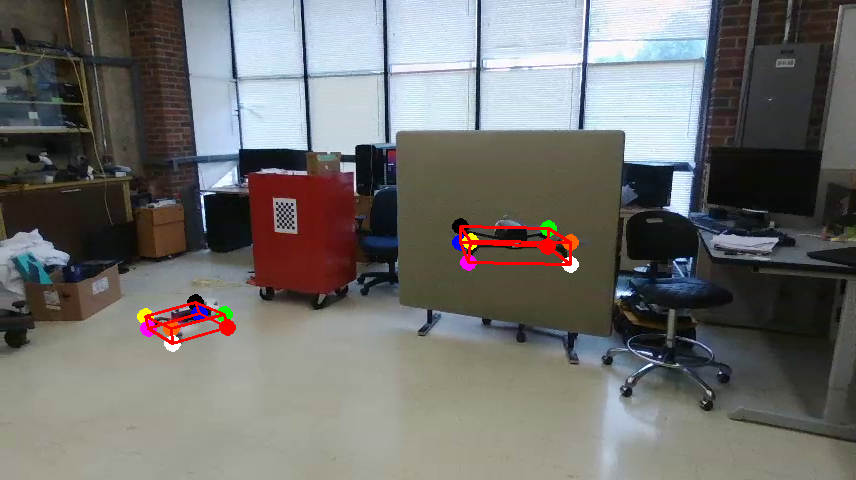
\includegraphics[width=0.49\textwidth]{images/pose_detection_picture.png}
    \end{center}
\end{multicols}

\newpage
\section*{Autonomous Robotic Vehicle Project (ARVP)}
I worked as part of a student club on making a fully autonomus custom underwater robot. I was focussed on improving state estimation accuracy, and lead full system tests in pools

\begin{multicols}{2}
    \subsection*{What did I do?}
    \begin{itemize}
        \item I lead and managed a small software team with another person
        \item I Implemented a Kalman filter to estimate an AUV's state by combining velocity and IMU sensor data 
        \item I Implemented a P-controller algorithm for autonomous vision-based underwater control
        \item I Troubleshooted network, CAN, and ROS communications live while leading full system tests
    \end{itemize}
    \subsection*{What technologies were used?}
    \begin{itemize}
        \item \textbf{ROS2} was used for easily making all of the different processes work together as a single system
        \item \textbf{Linux} and \textbf{Docker} were used to deploy our code onto the our robot, so that we could have a confidently consistent environment for developing and running code
        \item \textbf{Git} was used to manage code for an entire team
    \end{itemize}
    \vspace{10cm}
    \begin{center}
        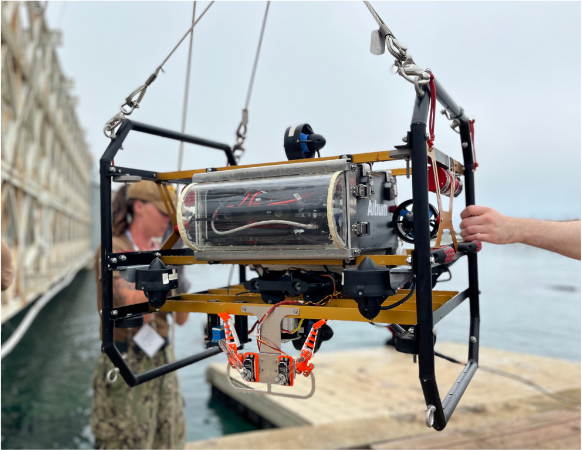
\includegraphics[width=0.49\textwidth]{images/arctos.png}
    \end{center}
\end{multicols}
    
    \section*{Wheeled Mobile Robot}
    I created a small wheeled wall-detecting mobile robot to learn more about mechatronics
    
\begin{multicols}{2}
    \subsection*{What did I do?}
    \begin{itemize}
        \item Designed, manufactured, and assembled a simple mobile robot capable of driving indoors 
        \item Sourced motors, motor drivers, sensors, and microcontrollers
        \item Designed and 3D printed a chassis to mount all electronics
    \end{itemize}
    \subsection*{What technologies were used?}
    \begin{itemize}
        \item \textbf{Onshape} was used to design all of the mounts and chassis of the robot
        \item \textbf{Arduino} was used to command the motor drivers and take in distance information from a range sensor   
    \end{itemize}
    \begin{center}
        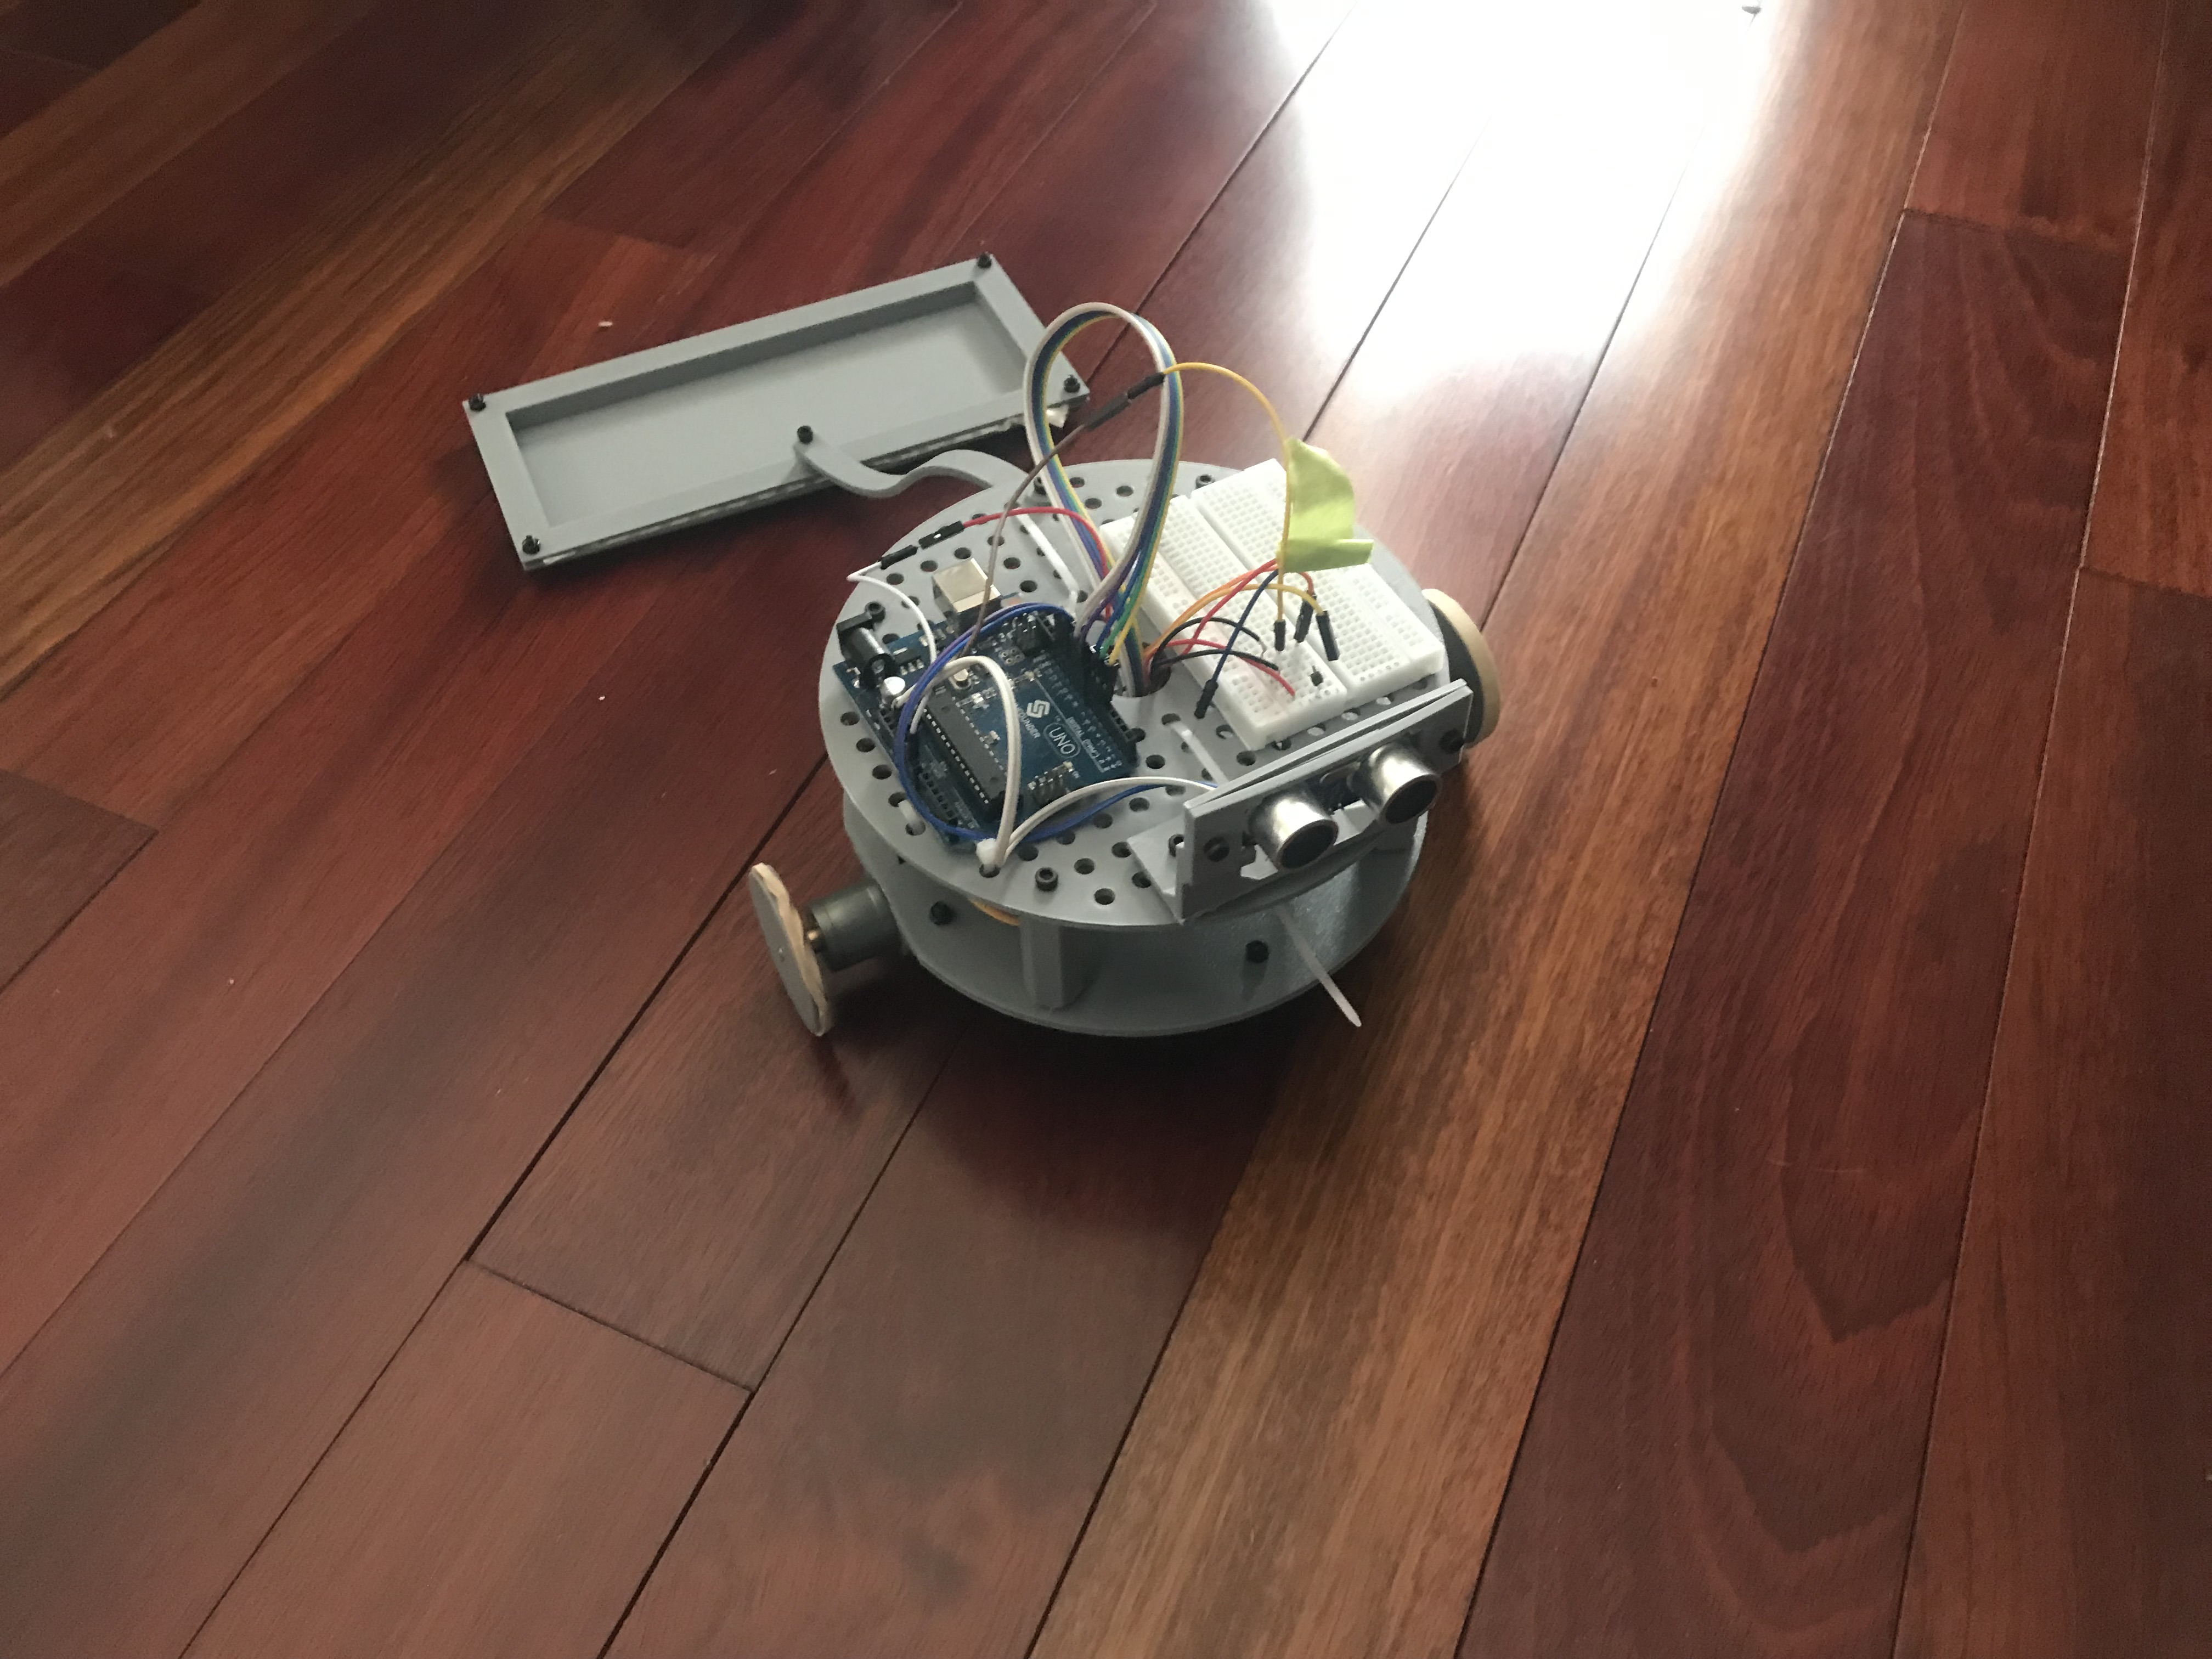
\includegraphics[width=0.49\textwidth, trim={25cm 30cm 40cm 10cm},clip]{images/mobile_robot.jpg}
    \end{center}
\end{multicols}

\newpage
\section*{Bimanual Force Controlled Robot}
I controlled a two-armed robot to clamp onto an object with a chosen force and move that object in 3D space

\begin{multicols}{2}
    \subsection*{What did I do?}
    \begin{itemize}
        \item Wrote a control algorithm for a bimanual 7DoF robot to control both a clamping force and the objects position simultaneously
        \item Used inverse kinematics library to convert world coordinates to joint angles
        \item Reviewed force control and dynamical systems control literature for arm robots
    \end{itemize}
    \subsection*{What technologies were used?}
    \begin{itemize}
        \item \textbf{ROS2} was used for easily making all of the different processes work together as a single system
        \item \textbf{Linux} and \textbf{Docker} were used to deploy our code onto the our robot, so that we could have a confidently consistent environment for developing and running code
    \end{itemize}
    \vspace{10cm}
    \begin{center}
        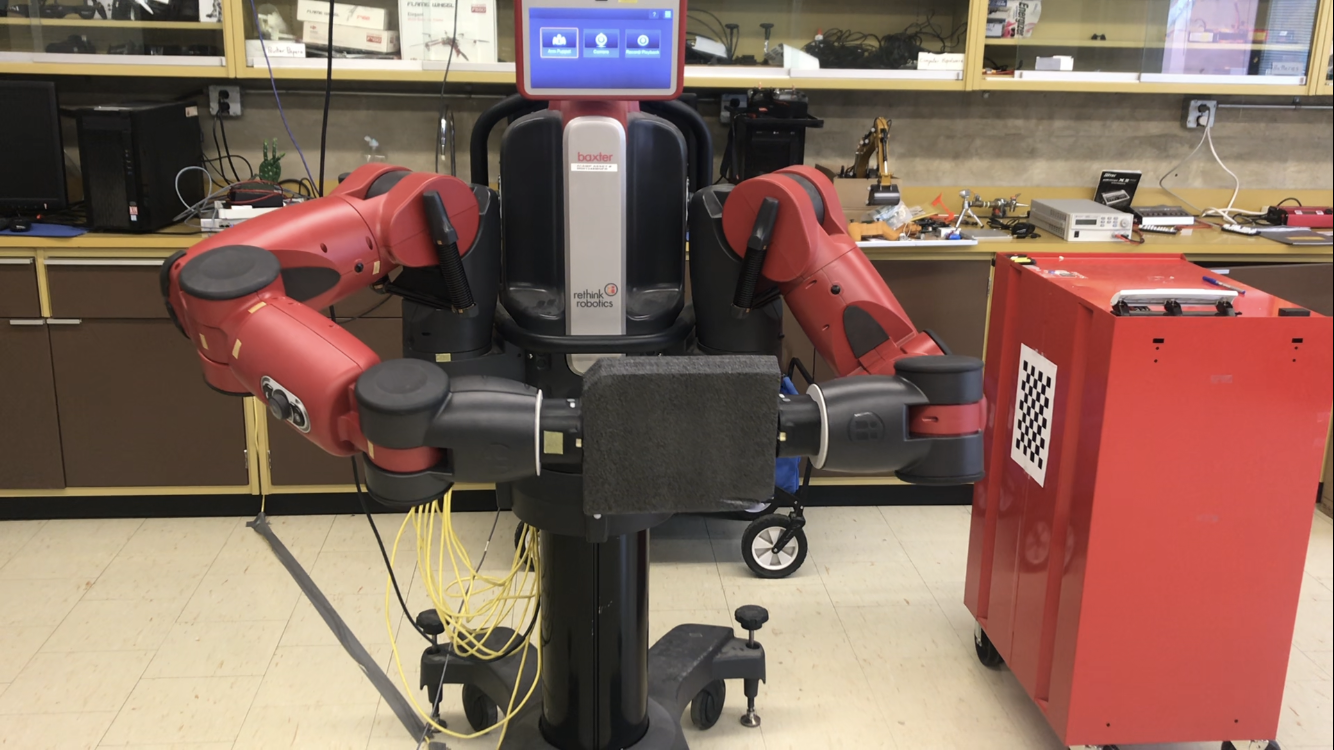
\includegraphics[width=0.49\textwidth]{images/baxter.png}
    \end{center}
\end{multicols}
    
\section*{Formula Student Rear Wing}
I lead a team to design a new rear wing for a formula student team 

\begin{multicols}{2}
    \subsection*{What did I do?}
    \begin{itemize}
        \item I designed a drag reduction system using servo motors capable of withstanding more than the expected aerodynamic loads
        \item I sourced and designed for all required hardware such as fasteners, actuators, and bearings
        \item I modelled the entire rear wing with all hardware and true geometry, as well as included the real range of motion to ensure nothing was overlooked before manufacturing
        \item I designed a rib and spar supported tail wing out of aluminum and carbon fiber
        \item I analyzed the design structurally for carbon fiber failures such as delamination, and for yielding and deflection requirements  
    \end{itemize}
    \subsection*{What technologies were used?}
    \begin{itemize}
        \item \textbf{SOLIDWORKS} was used for modelling all of the parts of the rear wing, as well as assembling this parts
        \item \textbf{Ansys Mechanical} was used to design the carbon fiber layup schedule as well as check for any potential structural failures in the assembly
    \end{itemize}
    \begin{center}
        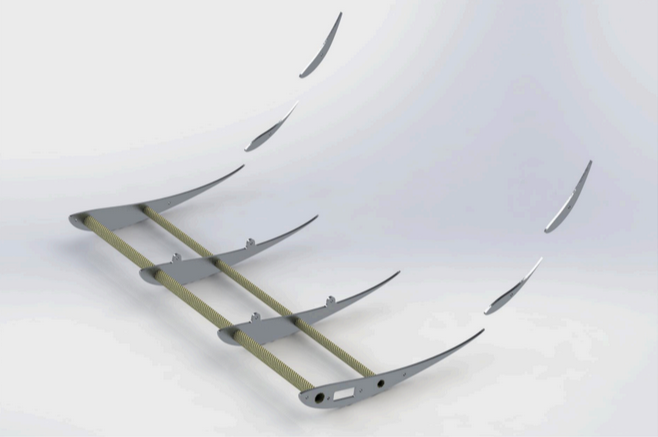
\includegraphics[width=0.49\textwidth]{images/rib_and_spar.png}
        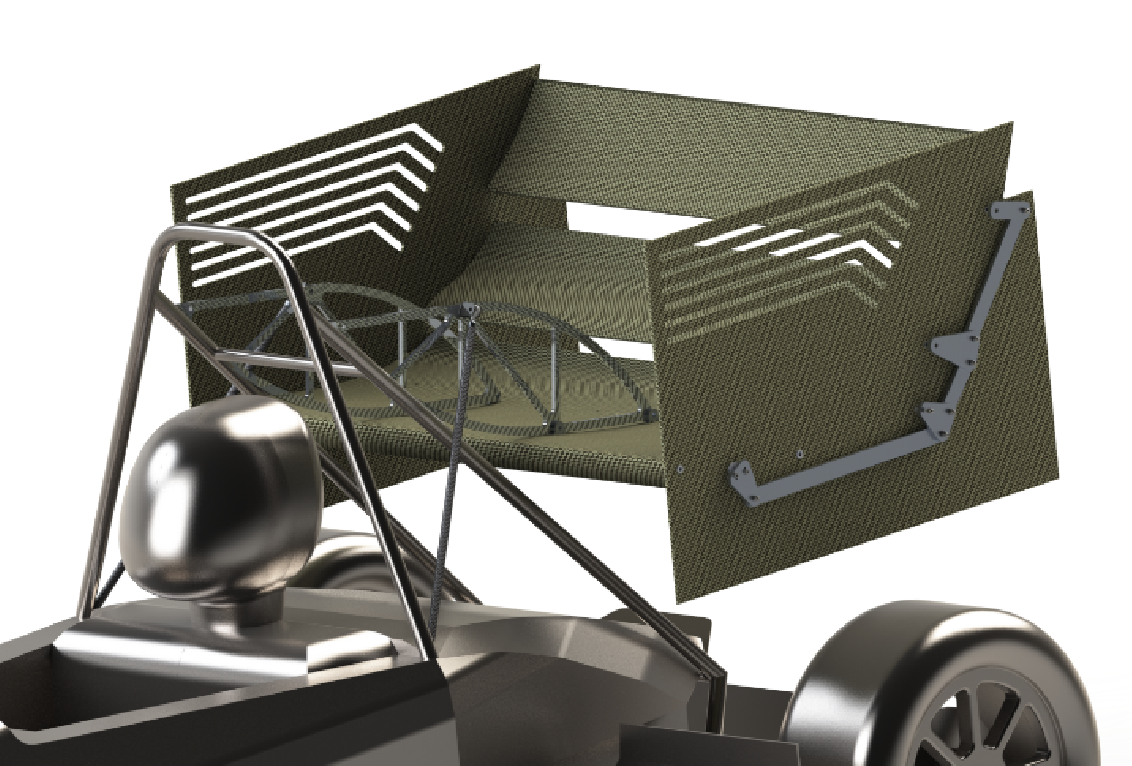
\includegraphics[width=0.49\textwidth]{images/integrated_rear_wing.png}
    \end{center}
\end{multicols}
        
\newpage
\begin{multicols}{2}
    [\section*{Automatic Ouiji Board}
    A group and I created a Ouiji board capable of automatially moving the planchette]
    
    \subsection*{What did I do?}
    \begin{itemize}
        \item I used an open source packages to programatically send G-code to a 3D printer gantry to create motion
        \item I then made functionality to convert words into GCode, so that other systems could interface simply with the hardware as needed
    \end{itemize}
    \subsection*{What technologies were used?}
    \begin{itemize}
        \item \textbf{Pronterface} was used to convert \textbf{Python} code into G-code
    \end{itemize}
    \begin{center}
        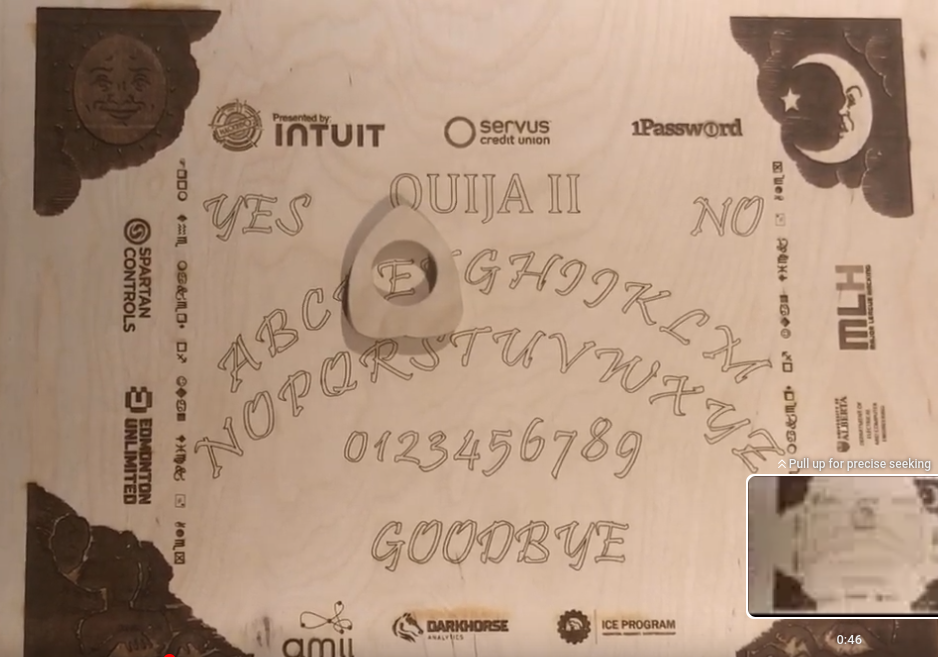
\includegraphics[width=0.49\textwidth]{images/ouija_board.png}
    \end{center}
\end{multicols}

\begin{multicols}{2}
    [\section*{Juan Wick}
    A group and I created a 2D game from scratch]
    
    \subsection*{What did I do?}
    \begin{itemize}
        \item I wrote actor control code to intelligently control enemies what would target the player
        \item I wrote a cinematic scene to control several actors in a cutscene
    \end{itemize}
    \subsection*{What technologies were used?}
    \begin{itemize}
        \item \textbf{C\#} was used for programming the behaviour of actors
        \item \textbf{Unity} was used as the game engine to simplify the game design process
    \end{itemize}    
    \begin{center}
        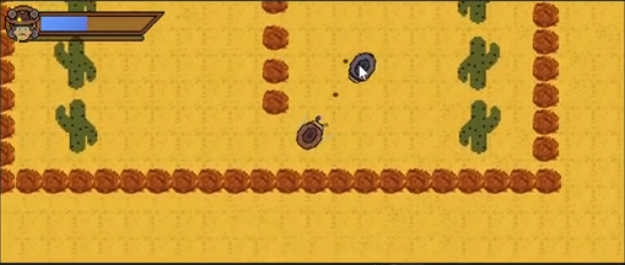
\includegraphics[width=0.49\textwidth, trim={0, 0, 8cm, 0}, clip]{images/juan_wick.png}
    \end{center}
\end{multicols}
    
    \end{document}